\section{Experimental results}

Tests were conducted by individually stressing some containers using Pumba and
checking the autoscaling response to those events.\\
In the reported example, the User Auth API and Restaurant Auth API have been
stressed. The initial load of the experiment is very low and, as shown in Figure
\ref{fig:cpu_before_user_auth}, there only is one replica per microservice and the
CPU usage is very low. Then, we stress User Auth API for a short amount of time and,
the autoscaler detects the load increase and creates a new replica (Figure
\ref{fig:cpu_after_user_auth}). After stressing that microservice, the load goes back
to a low level and, there is not enough time nor load for the autoscaler to create a
third replica; Restaurant Auth API still only has one replica since it has not been
stressed yet (Figure \ref{fig:cpu_before_restaurant_auth}). Eventually, we start to
stress
Restaurant Auth API and, as shown in Figure \ref{fig:cpu_after_restaurant_auth},
the autoscaler creates a new replica of that microservice. In the meantime, the
autoscaler also removes the additional replica previously created for User Auth API,
since its load decreased enough since then.\\
As a result, the system turned out to properly scale according to the given thresholds
and, this way, the load can be balanced across several replicas that in a potential
production system could be located
on different nodes, distributing the computation on more than one physical machine.

\begin{figure}
    \begin{center}
        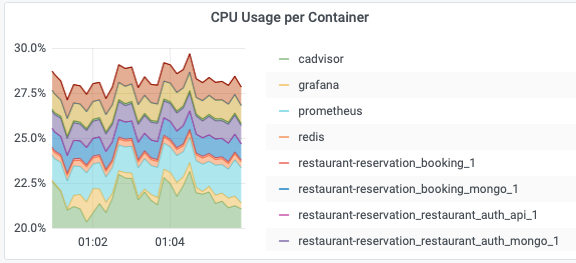
\includegraphics[width=8cm]{./images/cpu_before_user_auth.png}
    \end{center}
    \caption{CPU usage per container before stressing the User Auth API microservice.}
    \label{fig:cpu_before_user_auth}
\end{figure}

\begin{figure}
    \begin{center}
        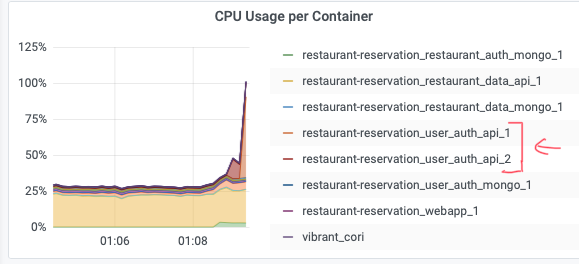
\includegraphics[width=8cm]{./images/cpu_after_user_auth.png}
    \end{center}
    \caption{CPU usage per container after stressing the User Auth API microservice.}
    \label{fig:cpu_after_user_auth}
\end{figure}

\begin{figure}
    \begin{center}
        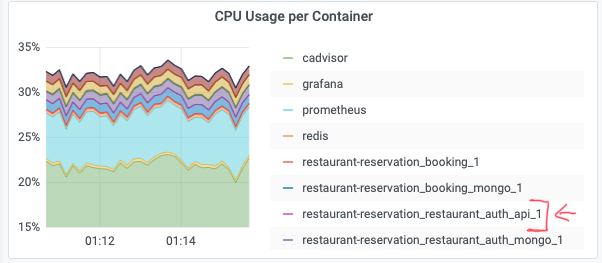
\includegraphics[width=8cm]{./images/cpu_before_restaurant_auth.png}
    \end{center}
    \caption{CPU usage per container before stressing the Restaurant Auth API microservice.}
    \label{fig:cpu_before_restaurant_auth}
\end{figure}

\begin{figure}
    \begin{center}
        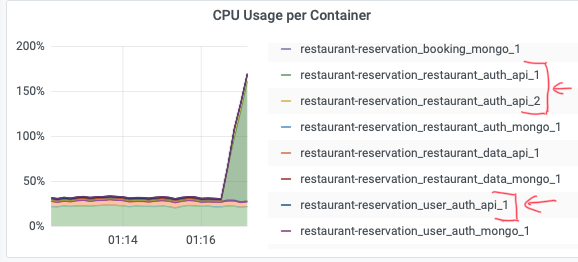
\includegraphics[width=8cm]{./images/cpu_after_restaurant_auth.png}
    \end{center}
    \caption{CPU usage per container after stressing the Restaurant Auth API microservice.}
    \label{fig:cpu_after_restaurant_auth}
\end{figure}
